\chapter{Introduzione ai Container}

\section*{Introduzione}
I container rappresentano una rivoluzione nel modo in cui sviluppiamo, distribuiamo ed eseguiamo applicazioni. Questo capitolo introduce i concetti fondamentali della containerizzazione, le differenze con le macchine virtuali tradizionali e l'architettura di Docker.

\section*{Obiettivi di apprendimento}
\begin{itemize}
    \item Comprendere cosa sono i container e come funzionano
    \item Confrontare container e macchine virtuali
    \item Conoscere i vantaggi della containerizzazione
    \item Capire l'architettura di Docker e i suoi componenti
    \item Identificare i casi d'uso appropriati per i container
\end{itemize}

\section{Cos'è un Container?}

\subsection{Definizione}
Un \textbf{container} è un'unità software standardizzata che impacchetta il codice e tutte le sue dipendenze in modo che l'applicazione possa essere eseguita in modo rapido e affidabile da un ambiente di computing a un altro.

\begin{tcolorbox}[colback=blue!10, colframe=blue!60, title=Analogia: Container di Spedizione]
Come i container di spedizione standardizzano il trasporto merci, i container software standardizzano il deployment di applicazioni:
\begin{itemize}
    \item \textbf{Dimensioni standard}: Formato uniforme e prevedibile
    \item \textbf{Portabilità}: Si spostano facilmente tra navi, treni, camion
    \item \textbf{Isolamento}: Il contenuto è separato dall'esterno
    \item \textbf{Efficienza}: Caricamento/scaricamento ottimizzato
\end{itemize}
\end{tcolorbox}

\subsection{Caratteristiche principali}
\begin{enumerate}
    \item \textbf{Isolamento}: Ogni container ha il proprio filesystem, processi, networking
    \item \textbf{Portabilità}: "Build once, run anywhere" - funziona su qualsiasi sistema
    \item \textbf{Leggerezza}: Condivide il kernel dell'host, avvio in secondi
    \item \textbf{Immutabilità}: L'immagine non cambia, deployment consistenti
    \item \textbf{Scalabilità}: Facilmente replicabile per gestire carico
\end{enumerate}

\section{Container vs Macchine Virtuali}

\subsection{Architettura a confronto}

\begin{figure}[h]
    \centering
    \begin{tikzpicture}[
        box/.style={rectangle, draw, minimum width=3cm, minimum height=0.8cm, align=center},
        layer/.style={box, fill=blue!20},
        vm/.style={box, fill=green!20},
        container/.style={box, fill=orange!20}
    ]
        % Virtual Machines
        \node[layer] (hw1) at (0,0) {Hardware};
        \node[layer] (os1) at (0,1) {OS Host};
        \node[layer] (hyp) at (0,2) {Hypervisor};
        \node[vm] (gos1) at (-1.5,3) {Guest OS};
        \node[vm] (gos2) at (0,3) {Guest OS};
        \node[vm] (gos3) at (1.5,3) {Guest OS};
        \node[vm] (app1) at (-1.5,4) {App A};
        \node[vm] (app2) at (0,4) {App B};
        \node[vm] (app3) at (1.5,4) {App C};

        \node[above=0.3cm of app2] {\textbf{Virtual Machines}};

        % Containers
        \node[layer] (hw2) at (6,0) {Hardware};
        \node[layer] (os2) at (6,1) {OS Host};
        \node[layer] (docker) at (6,2) {Docker Engine};
        \node[container] (cnt1) at (4.5,3.5) {App A\\Libs};
        \node[container] (cnt2) at (6,3.5) {App B\\Libs};
        \node[container] (cnt3) at (7.5,3.5) {App C\\Libs};

        \node[above=0.3cm of cnt2] {\textbf{Containers}};
    \end{tikzpicture}
    \caption{Architettura: Virtual Machines vs Containers}
\end{figure}

\subsection{Differenze chiave}

\begin{table}[h]
\centering
\begin{tabular}{|l|l|l|}
\hline
\textbf{Caratteristica} & \textbf{Virtual Machine} & \textbf{Container} \\
\hline
Dimensione & GB (include intero OS) & MB (solo app + dipendenze) \\
Avvio & Minuti & Secondi \\
Performance & Overhead hypervisor & Quasi native \\
Isolamento & Completo (hardware) & A livello processo \\
Portabilità & Limitata (formato VM) & Eccellente (standard OCI) \\
Densità & Decine per host & Centinaia per host \\
\hline
\end{tabular}
\caption{Confronto VM vs Container}
\end{table}

\subsection{Virtual Machines}
\textbf{Vantaggi}:
\begin{itemize}
    \item Isolamento completo a livello hardware
    \item Esecuzione di OS diversi sullo stesso host
    \item Sicurezza superiore (separazione hypervisor)
    \item Supporto per applicazioni legacy
\end{itemize}

\textbf{Svantaggi}:
\begin{itemize}
    \item Overhead significativo (ogni VM ha un OS completo)
    \item Avvio lento (boot del sistema operativo)
    \item Consumo elevato di risorse (RAM, CPU, disco)
    \item Portabilità limitata tra hypervisor diversi
\end{itemize}

\subsection{Containers}
\textbf{Vantaggi}:
\begin{itemize}
    \item Leggerezza: condividono il kernel dell'host
    \item Avvio istantaneo (secondi)
    \item Alta densità: centinaia di container per server
    \item Portabilità: funzionano ovunque ci sia Docker
    \item Efficienza: minor spreco di risorse
    \item CI/CD: integrazione perfetta in pipeline DevOps
\end{itemize}

\textbf{Svantaggi}:
\begin{itemize}
    \item Isolamento meno robusto delle VM
    \item Stesso kernel dell'host (no OS diversi)
    \item Sicurezza: vulnerabilità kernel colpisce tutti i container
    \item Non adatti per applicazioni che richiedono kernel diverso
\end{itemize}

\begin{nota}
Container e VM non sono mutualmente esclusivi. Molte architetture moderne usano \textbf{container dentro VM}: le VM forniscono isolamento hardware, i container portano portabilità e densità.
\end{nota}

\section{Vantaggi della Containerizzazione}

\subsection{1. Portabilità e Consistenza}

\begin{tcolorbox}[colback=green!10, colframe=green!60, title=Problema: "Works on my machine"]
\textbf{Scenario tradizionale}:
\begin{itemize}
    \item Sviluppo su macOS
    \item Staging su Ubuntu 20.04
    \item Produzione su CentOS 8
    \item Risultato: bug dipendenti dall'ambiente
\end{itemize}

\textbf{Soluzione con container}:
\begin{itemize}
    \item Immagine Docker identica ovunque
    \item Stesso runtime, librerie, dipendenze
    \item Risultato: comportamento prevedibile
\end{itemize}
\end{tcolorbox}

\subsection{2. Microservizi e Scalabilità}

I container sono ideali per architetture a microservizi:
\begin{itemize}
    \item \textbf{Isolamento}: Ogni servizio in un container separato
    \item \textbf{Scalabilità indipendente}: Scala solo i servizi sotto carico
    \item \textbf{Deployment incrementale}: Aggiorna un servizio alla volta
    \item \textbf{Resilienza}: Fallimento di un container non compromette il sistema
\end{itemize}

\begin{lstlisting}[caption=Esempio: Stack microservizi]
# Frontend
Container 1: React app (3 repliche)

# Backend API
Container 2: Node.js API (5 repliche)
Container 3: Python ML service (2 repliche)

# Database
Container 4: PostgreSQL (1 replica master)
Container 5: Redis cache (2 repliche)
\end{lstlisting}

\subsection{3. DevOps e CI/CD}

I container accelerano il ciclo di sviluppo:

\begin{enumerate}
    \item \textbf{Sviluppo}: Ambiente identico per tutti i developer
    \item \textbf{Testing}: Test automatici in container isolati
    \item \textbf{Build}: Immagine Docker come artifact immutabile
    \item \textbf{Deployment}: Push immagine su registry, pull in produzione
    \item \textbf{Rollback}: Ritorna alla versione precedente in secondi
\end{enumerate}

\begin{figure}[h]
    \centering
    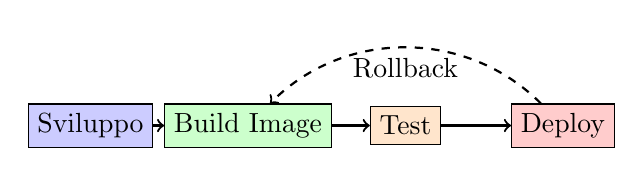
\begin{tikzpicture}[node distance=2cm]
        \node[draw, rectangle, fill=blue!20] (dev) {Sviluppo};
        \node[draw, rectangle, fill=green!20, right of=dev] (build) {Build Image};
        \node[draw, rectangle, fill=orange!20, right of=build] (test) {Test};
        \node[draw, rectangle, fill=red!20, right of=test] (deploy) {Deploy};

        \draw[->, thick] (dev) -- (build);
        \draw[->, thick] (build) -- (test);
        \draw[->, thick] (test) -- (deploy);
        \draw[->, thick, dashed] (deploy) to[bend right=45] node[below] {Rollback} (build);
    \end{tikzpicture}
    \caption{Pipeline CI/CD con Docker}
\end{figure}

\subsection{4. Efficienza delle Risorse}

\begin{table}[h]
\centering
\begin{tabular}{|l|r|r|r|}
\hline
\textbf{Metrica} & \textbf{VM} & \textbf{Container} & \textbf{Risparmio} \\
\hline
Memoria per istanza & 2 GB & 100 MB & 95\% \\
Tempo avvio & 60 sec & 2 sec & 97\% \\
Istanze per server & 10 & 100 & 10x \\
Costo cloud mensile & \$500 & \$50 & 90\% \\
\hline
\end{tabular}
\caption{Confronto efficienza risorse (valori medi)}
\end{table}

\section{Architettura Docker}

\subsection{Componenti principali}

\begin{figure}[h]
    \centering
    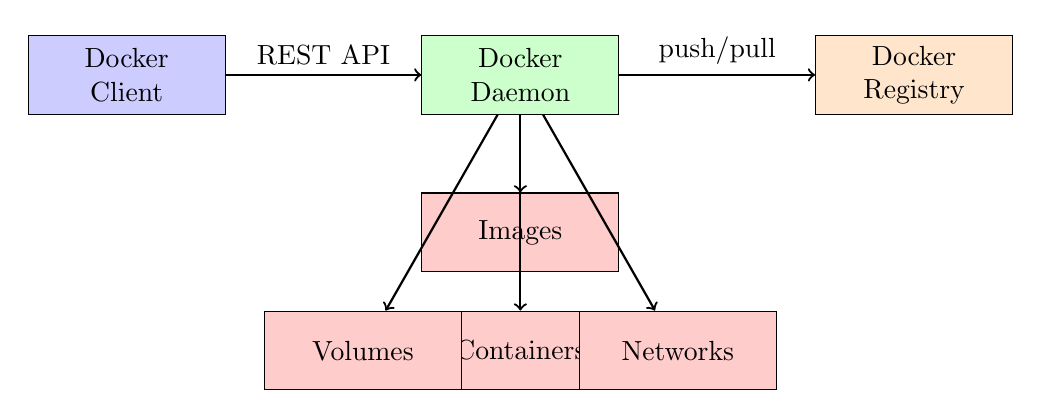
\begin{tikzpicture}[
        component/.style={rectangle, draw, minimum width=2.5cm, minimum height=1cm, align=center},
        arrow/.style={->, thick}
    ]
        % Docker Client
        \node[component, fill=blue!20] (client) at (0,0) {Docker\\Client};

        % Docker Daemon
        \node[component, fill=green!20] (daemon) at (5,0) {Docker\\Daemon};

        % Registry
        \node[component, fill=orange!20] (registry) at (10,0) {Docker\\Registry};

        % Objects
        \node[component, fill=red!20] (images) at (5,-2) {Images};
        \node[component, fill=red!20] (containers) at (5,-3.5) {Containers};
        \node[component, fill=red!20] (volumes) at (3,-3.5) {Volumes};
        \node[component, fill=red!20] (networks) at (7,-3.5) {Networks};

        % Arrows
        \draw[arrow] (client) -- node[above] {REST API} (daemon);
        \draw[arrow] (daemon) -- node[above] {push/pull} (registry);
        \draw[arrow] (daemon) -- (images);
        \draw[arrow] (daemon) -- (containers);
        \draw[arrow] (daemon) -- (volumes);
        \draw[arrow] (daemon) -- (networks);
    \end{tikzpicture}
    \caption{Architettura Docker}
\end{figure}

\subsubsection{Docker Client}
Interfaccia utente per interagire con Docker:
\begin{itemize}
    \item Comando \texttt{docker}: CLI principale
    \item Invia comandi al Docker Daemon via REST API
    \item Può connettersi a daemon remoti
\end{itemize}

\begin{lstlisting}[language=bash]
# Esempi di comandi client
$ docker run nginx
$ docker ps
$ docker build -t myapp .
$ docker push myapp:latest
\end{lstlisting}

\subsubsection{Docker Daemon (dockerd)}
Il cuore di Docker che gestisce:
\begin{itemize}
    \item Building, running, distributing container
    \item Gestione immagini, container, reti, volumi
    \item Comunicazione con registry per push/pull
    \item Esposizione REST API per client
\end{itemize}

\subsubsection{Docker Registry}
Repository per immagini Docker:
\begin{itemize}
    \item \textbf{Docker Hub}: Registry pubblico ufficiale
    \item \textbf{Registry privati}: Harbor, Artifactory, AWS ECR, GCP GCR
    \item \textbf{Self-hosted}: Registry Docker open source
\end{itemize}

\subsection{Oggetti Docker}

\subsubsection{Immagini}
Template \textbf{read-only} per creare container:
\begin{itemize}
    \item File system stratificato (layers)
    \item Definite da un Dockerfile
    \item Versionabili con tags (latest, v1.0, stable)
    \item Riutilizzabili e componibili
\end{itemize}

\begin{lstlisting}[caption=Struttura immagine a layer]
Layer 5: App code (Python)         10 MB
Layer 4: pip install requirements   50 MB
Layer 3: Python 3.9                 100 MB
Layer 2: OS libraries (Ubuntu)      30 MB
Layer 1: Base layer                 5 MB
----------------------------------------
Total:                              195 MB
\end{lstlisting}

\subsubsection{Container}
Istanza \textbf{eseguibile} di un'immagine:
\begin{itemize}
    \item Processo isolato con proprio filesystem
    \item Layer writable sopra l'immagine
    \item Effimero: può essere fermato, rimosso, ricreato
    \item Configurabile: variabili ambiente, porte, volumi
\end{itemize}

\subsubsection{Volumi}
Persistenza dati al di fuori del container:
\begin{itemize}
    \item Sopravvivono alla cancellazione del container
    \item Condivisibili tra più container
    \item Gestiti da Docker (ottimizzazione I/O)
\end{itemize}

\subsubsection{Reti}
Comunicazione tra container e verso l'esterno:
\begin{itemize}
    \item \textbf{Bridge}: Rete privata isolata (default)
    \item \textbf{Host}: Usa network stack dell'host
    \item \textbf{Overlay}: Multi-host networking (Swarm/Kubernetes)
    \item \textbf{None}: Nessun networking
\end{itemize}

\section{Tecnologie Sottostanti}

\subsection{Namespace Linux}
Isolamento delle risorse del sistema:
\begin{itemize}
    \item \textbf{PID}: Albero processi isolato
    \item \textbf{Network}: Stack di rete separato
    \item \textbf{Mount}: Filesystem isolato
    \item \textbf{UTS}: Hostname e domain name
    \item \textbf{IPC}: Inter-process communication
    \item \textbf{User}: Mapping UID/GID
\end{itemize}

\subsection{Control Groups (cgroups)}
Limitazione e accounting delle risorse:
\begin{itemize}
    \item CPU: Limiti di utilizzo processore
    \item Memoria: Limiti RAM e swap
    \item I/O: Bandwidth disco
    \item Network: Bandwidth rete
\end{itemize}

\begin{lstlisting}[language=bash, caption=Esempio: Limitare risorse container]
# Limita a 1 CPU e 512 MB RAM
$ docker run --cpus="1.0" --memory="512m" nginx
\end{lstlisting}

\subsection{Union File System}
Filesystem stratificato:
\begin{itemize}
    \item \textbf{OverlayFS}: Default su Linux moderno
    \item \textbf{AUFS}: Legacy Ubuntu
    \item \textbf{Btrfs/ZFS}: COW filesystem avanzati
\end{itemize}

\textbf{Vantaggi}:
\begin{itemize}
    \item Condivisione layer tra immagini (risparmio spazio)
    \item Build veloce (caching layer)
    \item Pull efficiente (solo layer mancanti)
\end{itemize}

\section{Storia ed Evoluzione}

\subsection{Timeline}
\begin{itemize}
    \item \textbf{1979}: chroot (primi concetti di isolamento)
    \item \textbf{2000}: FreeBSD Jails
    \item \textbf{2005}: OpenVZ, Solaris Zones
    \item \textbf{2008}: LXC (Linux Containers)
    \item \textbf{2013}: Docker Inc. lancia Docker
    \item \textbf{2014}: Kubernetes (orchestrazione Google)
    \item \textbf{2015}: Docker Compose
    \item \textbf{2017}: Docker Swarm mode
    \item \textbf{2020}: Docker supporta Windows containers
    \item \textbf{2021}: containerd diventa CNCF graduated project
\end{itemize}

\subsection{Open Container Initiative (OCI)}
Standardizzazione del formato container:
\begin{itemize}
    \item \textbf{Image spec}: Formato immagine universale
    \item \textbf{Runtime spec}: Specifiche esecuzione container
    \item \textbf{Distribution spec}: Distribuzione via registry
\end{itemize}

\textbf{Implementazioni OCI}:
\begin{itemize}
    \item Docker
    \item containerd
    \item CRI-O (Kubernetes)
    \item Podman (Red Hat)
\end{itemize}

\section{Casi d'Uso}

\subsection{Quando usare i container}

\textbf{Ideali per}:
\begin{itemize}
    \item Microservizi e API stateless
    \item Applicazioni web moderne (MERN, LAMP, MEAN)
    \item CI/CD e ambienti di sviluppo
    \item Batch processing e job worker
    \item Funzioni serverless (AWS Lambda usa container)
\end{itemize}

\textbf{Non ideali per}:
\begin{itemize}
    \item Applicazioni GUI desktop
    \item Kernel modules e driver
    \item Applicazioni che richiedono hardware specifico
    \item Database con I/O intensivo (meglio VM o bare metal)
\end{itemize}

\subsection{Esempi reali}

\begin{tcolorbox}[colback=blue!10, colframe=blue!60, title=Caso 1: E-commerce Platform]
\textbf{Architettura}:
\begin{itemize}
    \item 10 container frontend (React)
    \item 20 container backend (Node.js API)
    \item 5 container cart service (Python)
    \item 3 container payment gateway
    \item 2 database (PostgreSQL + Redis)
\end{itemize}

\textbf{Risultati}:
\begin{itemize}
    \item Deploy 50 volte al giorno (vs 1 volta/settimana)
    \item Downtime ridotto 99\%
    \item Costi cloud -60\%
\end{itemize}
\end{tcolorbox}

\begin{tcolorbox}[colback=green!10, colframe=green!60, title=Caso 2: Machine Learning Pipeline]
\textbf{Setup}:
\begin{itemize}
    \item Container data ingestion (Kafka)
    \item Container preprocessing (Spark)
    \item Container training (TensorFlow GPU)
    \item Container model serving (Flask API)
\end{itemize}

\textbf{Vantaggi}:
\begin{itemize}
    \item Riproducibilità esperimenti
    \item Scalabilità training parallelizzato
    \item Deployment modelli senza downtime
\end{itemize}
\end{tcolorbox}

\section*{Best Practices}

\begin{tcolorbox}[colback=yellow!10, colframe=orange!60, title=Best Practices Iniziali]
\begin{enumerate}
    \item \textbf{Un processo per container}: Non usare supervisord/systemd
    \item \textbf{Immutabilità}: Mai modificare container in esecuzione
    \item \textbf{Stateless}: Stato persistente su volumi esterni
    \item \textbf{Logging}: Output su stdout/stderr, non file
    \item \textbf{Configurazione}: Usa variabili ambiente, non file config
    \item \textbf{Sicurezza}: Non eseguire come root se evitabile
\end{enumerate}
\end{tcolorbox}

\section*{Errori Comuni}

\begin{attenzione}
\textbf{Errori da evitare}:
\begin{itemize}
    \item Trattare container come VM (ssh, multiple process)
    \item Salvare dati importanti nel container filesystem
    \item Immagini enormi (GB) con software inutile
    \item Eseguire tutto come root
    \item Hardcodare configurazione nel Dockerfile
    \item Non versionare immagini (usare sempre tags)
\end{itemize}
\end{attenzione}

\section*{Esercizi}

\begin{enumerate}
    \item Disegna un diagramma che confronta l'architettura di VM e container, evidenziando le differenze di layer.

    \item Spiega con un esempio concreto come i container risolvono il problema "works on my machine".

    \item Identifica 3 applicazioni nella tua scuola/azienda che potrebbero beneficiare della containerizzazione. Motiva la scelta.

    \item Calcola il risparmio teorico: hai 50 applicazioni che richiedono 1GB RAM ciascuna. Confronta il costo di:
    \begin{itemize}
        \item VM (overhead 2GB per VM)
        \item Container (overhead 100MB per container)
    \end{itemize}

    \item Ricerca: trova 3 aziende famose che usano Docker in produzione e scopri come lo utilizzano.
\end{enumerate}

\section*{Quiz di Verifica}

\begin{enumerate}
    \item \textbf{Vero/Falso}: I container condividono il kernel dell'host.

    \item \textbf{Vero/Falso}: Un container può eseguire Windows su un host Linux.

    \item Quale componente Docker gestisce la comunicazione tra client e daemon?
    \begin{itemize}
        \item a) Registry
        \item b) REST API
        \item c) Dockerfile
        \item d) Namespace
    \end{itemize}

    \item Qual è il vantaggio principale dei layer nelle immagini Docker?

    \item Quando preferiresti una VM a un container?
\end{enumerate}

\section*{Riepilogo Concetti Chiave}

\begin{tcolorbox}[colback=gray!10, colframe=black!60, title=Concetti Fondamentali]
\begin{itemize}
    \item I \textbf{container} sono unità software leggere e portabili
    \item \textbf{Vantaggi vs VM}: Più leggeri, avvio rapido, alta densità
    \item \textbf{Docker} è la piattaforma leader per containerizzazione
    \item \textbf{Architettura}: Client, Daemon, Registry, Objects
    \item \textbf{Tecnologie}: Namespace, cgroups, Union FS
    \item \textbf{Portabilità}: Build once, run anywhere
    \item \textbf{DevOps}: CI/CD, microservizi, scalabilità
\end{itemize}
\end{tcolorbox}

\section*{Prossimi Passi}

Nel prossimo capitolo esploreremo:
\begin{itemize}
    \item Installazione Docker su diversi sistemi operativi
    \item Comandi base: run, ps, images, stop, rm
    \item Gestione del ciclo di vita dei container
    \item Debugging e troubleshooting
\end{itemize}

\section*{Riferimenti}

\begin{itemize}
    \item Docker Official Docs: \url{https://docs.docker.com}
    \item OCI Specifications: \url{https://opencontainers.org}
    \item Linux Namespaces: \url{https://man7.org/linux/man-pages/man7/namespaces.7.html}
    \item cgroups: \url{https://www.kernel.org/doc/Documentation/cgroup-v2.txt}
    \item Docker Blog: \url{https://www.docker.com/blog}
    \item CNCF: \url{https://www.cncf.io}
\end{itemize}
